\section{Sequentielle Logik}
\subsection{Abgrenzung zur Kombinatorischen Logik}
\begin{center}
    \begin{minipage}[t]{0.45\linewidth}
        \paragraph{Kombinatorische Schaltung}
        Output hängt von Inputs und Verknüpfungen ab.
	Das System hat keinen Speicher.
    \end{minipage}
    \hfill
    \begin{minipage}[t]{0.45\linewidth}
        \paragraph{Sequentielle Schaltung}
        Output hängt vom Zustand ab.
	Benötigt einen Speicher.
	Die Speicher-Ausgänge sind oft rückgekoppelt.
    \end{minipage}
\end{center}
\subsection{D-Flip-Flop}
\begin{minipage}{0.45\linewidth}
	\begin{center}
		\includegraphics[width=0.5\linewidth]{images/dflip.png}
	\end{center}
\end{minipage}
\begin{minipage}{0.45\linewidth}
	Wert am Eingang D wird gespeichert und an den Ausgang Q übertragen, wenn C von 0 auf 1 wechselt.
\end{minipage}
\begin{center}
\begin{equation*}
	Q_{n+1} = D \quad \text{wenn} \quad CLK 0 \rightarrow 1
\end{equation*}
	$n$ Flip-Flops können $2^n$ Zustände annehmen.
\end{center}

\subsection{Clock Signal}
	\begin{minipage}{0.45\linewidth}
		\begin{center}
            	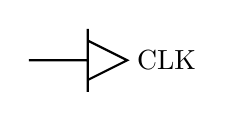
\begin{tikzpicture}
                	\draw[thick] (-0.75, 0) -- (0,0)
                    	(0,0.4) -- (0,-0.4)
                    	(0,0.25) -- (0.5,0) -- (0,-0.25);
                	\node[] at (1, 0) {CLK};
            	\end{tikzpicture}
        	\end{center}
        Input beim Übergang von \emph{$0 \rightarrow 1$} von CLK wirksam.
        \begin{center}
		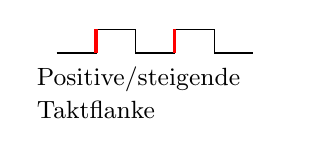
\begin{tikzpicture}
                	\draw (0,0) -- (0.5, 0) -- (0.5, 0.3) -- (1, 0.3) -- (1, 0) -- (1.5, 0) -- (1.5, 0.3) -- (2, 0.3) -- (2, 0) -- (2.5, 0);
                	\draw[very thick, red] (0.5, 0) -- (0.5, 0.3) (1.5, 0) -- (1.5, 0.3);
                	\node[text width = 30mm] at (1.25, -0.5) {\small Positive/steigende Taktflanke};
            	\end{tikzpicture}
        \end{center}
    	\end{minipage}
    	\hfill
    	\begin{minipage}{0.45\linewidth}
        	\begin{center}
            	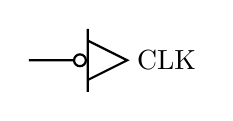
\begin{tikzpicture}
                	\draw[thick] (-0.75, 0) -- (0,0)
                    	(0,0.4) -- (0,-0.4)
                    	(0,0.25) -- (0.5,0) -- (0,-0.25);
                	\draw[thick, fill = white] (-0.1,0) circle [radius = 0.75mm];
                	\node[] at (1, 0) {CLK};
            	\end{tikzpicture}
        	\end{center}
        	Input beim Übergang von \emph{$1 \rightarrow 0$} von CLK wirksam.
        	\begin{center}
            		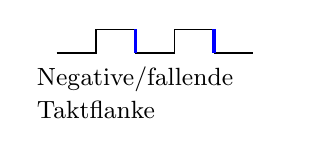
\begin{tikzpicture}
                		\draw (0,0) -- (0.5, 0) -- (0.5, 0.3) -- (1, 0.3) -- (1, 0) -- (1.5, 0) -- (1.5, 0.3) -- (2, 0.3) -- (2, 0) -- (2.5, 0);
                		\draw[very thick, blue] (1, 0.3) -- (1, 0) (2, 0.3) -- (2, 0);
                		\node[text width = 30mm] at (1.25, -0.5) {\small Negative/fallende Taktflanke};
            		\end{tikzpicture}
        	\end{center}
    	\end{minipage}

\subsection{Frequenzteiler}
Kaskadieren von T-Flipflops führt zu einer Frequenzreduktion von CLK um den Faktor 2.
\begin{center}
    \begin{minipage}{0.55\linewidth}
        \begin{circuit}[0.25]
            \ctikzset{multipoles/flipflop/clock wedge size=0.5}
            \node[tFfmin] (t1) {};
            \node[tFfmin, right = 6mm of t1] (t2) {};
            \node[tFfmin, right = 6mm of t2] (t3) {};
        
            \node[font = \footnotesize, left = 0.9mm of t1.pin 2] (clk) {\cirin{CLK}}; 
        
            \begin{pgfonlayer}{tl1}
                \node[circ] (nex1) at ($(t1.pin 6)!0.5!(t2.pin 1)$) {};
                \node[circ] (nex2) at ($(t2.pin 6)!0.5!(t3.pin 1)$) {};
            \end{pgfonlayer}
            \node[above = 4mm of nex1, font = \footnotesize] (q0) {$Q_0$};
            \node[above = 4mm of nex2, font = \footnotesize] (q1) {$Q_1$};
            \node[above = 4.5mm of t3.pin 6, font = \footnotesize] (q2) {$Q_2$};
        
            \draw (clk) -- (t1.pin 2);
            \draw (t1.pin 6) -- (nex1) |- (t2.pin 2);
            \draw (t2.pin 6) -- (nex2) |- (t3.pin 2);
            \draw (nex2) -- (q1);
            \path[draw] (nex1) -- (q0) node[midway, left, font = \footnotesize] {};  
            \path[draw] (t3.pin 6) -- (q2) node[midway, right, font = \footnotesize] {}; 
        \end{circuit}
    \end{minipage}
    \hfill
    \begin{minipage}{0.4\linewidth}
        \begin{center}
            \begin{tikzpicture}
                \coordinate[label = {[font = \footnotesize]180:\cirin{CLK}}](clk) at (0,0.5);
                \coordinate[label = {[font = \footnotesize]180:$Q_0$}](q1) at (0,0);
                \coordinate[label = {[font = \footnotesize]180:$Q_1$}](q2) at (0,-0.5);

                \draw[thick] (clk) --++(0:0.4) --++(90:0.2) coordinate(f1t) --++(0:0.4) --++(270:0.2) --++(0:0.4) --++(90:0.2) coordinate(f2t) --++(0:0.4) --++(270:0.2) --++(0:0.4) --++(90:0.2)coordinate(f3t) --++(0:0.05);
                \draw[thick] (q1) --++(0:0.4) --++(90:0.2) --++(0:0.8) --++(270:0.2)coordinate(f2b) --++(0:0.8) --++(90:0.2) --++(0:0.05);
                \draw[thick] (q2) --++(0:0.4) coordinate(f1b) --++(90:0.2) --++(0:1.6) --++(270:0.2)coordinate(f3b) --++(0:0.05);

                \begin{pgfonlayer}{bg}
                    \fill[red!50, rounded corners = 2pt] ($(f1t) +(-0.1,0.1)$) rectangle ($(f1b) + (0.1, -0.1)$);
                    \fill[red!50, rounded corners = 2pt] ($(f2t) +(-0.1,0.1)$) rectangle ($(f2b) + (0.1, -0.1)$);
                    \fill[red!50, rounded corners = 2pt] ($(f3t) +(-0.1,0.1)$) rectangle ($(f3b) + (0.1, -0.1)$);
                \end{pgfonlayer}
            \end{tikzpicture}
        \end{center}
    \end{minipage}
\end{center}

\subsection{Arten von Sequentiellen Schaltungen}
\subsubsection{Counter}
\begin{itemize}
	\item Einfache Form der sequentiellen Logik (endlicher Zustandsautomat).
	\item Zustandswechsel bei steigender Taktflanke.
	\item Die Reihenfolge der Zustände kann nicht von aussen beeinflusst werden.
	\item Die Ausgänge hängen nur vom internen Zustand ab.
\end{itemize}
\begin{center}
	\includegraphics[width=1\linewidth]{images/counter.png}
\end{center}
\subsubsection{Finite State Machine}
\begin{itemize}
	\item Enthält Speicher.
	\item Der Ausgang ist abhängig vom Input und dem Status des Speichers.
	\item Der FF-Ausgangswert entspricht dem Zustand des Automaten.
	\item Bei jedem Takt-Signal (Clock) wird der Speicher neu geladen.
\end{itemize}
\begin{center}
	\includegraphics[width=1\linewidth]{images/FSM.png}
\end{center}
\subsubsection{Shift Register}
\begin{itemize}
	\item Enthält mehrere in Reihe geschaltete FFs.
	\item Die Eingänge können seriell oder parallel sein.
	\item Die Ausgänge können seriell oder parallel sein.
	\item Es kann Rückkopplungen enthalten oder nicht.
\end{itemize}
\begin{center}
	\includegraphics[width=1\linewidth]{images/shiftregister.png}
\end{center}

\subsection{Register}
\subsubsection{Parallel Register}
\begin{itemize}
	\item Ein- und Ausgänge sind parallel.
	\item Beispiel dafür: 8-bit Register.
	\item Inputs \quad in7 - in0 -> Werden bei steigender Flanke gespeichert.
	\item Outputs \quad out7 - out0.
	\item Schnellster Speicher im Prozessor.
\end{itemize}
\begin{center}
	\includegraphics[width=1\linewidth]{images/8bitreg.png}
\end{center}
\subsubsection{Schieberegister}
\begin{itemize}
	\item Jeder Ausgang ist mit dem Eingang verbunden.
	\item Zustand des Ausgangs wird zum Eingang rübergeschoben bei jeder Flanke.
\end{itemize}
\begin{center}
	\includegraphics[width=1\linewidth]{images/schiebereg.png}
\end{center}
\begin{center}
	\includegraphics[width=1\linewidth]{images/schieberegtime.png}
\end{center}

\subsubsection{Beispiel für Zustandsdiagramm}
\begin{align*}
	\includegraphics[width=1\linewidth]{images/zustandsdiagramm.png}
\end{align*}